% Figure blocks for dissertation
% Source data: results/results.csv
% Generated plots live under ../plots/

% -----------------------------
% Chapter 5 figures (evaluation)
% -----------------------------

\begin{figure}[htbp]
    \centering
    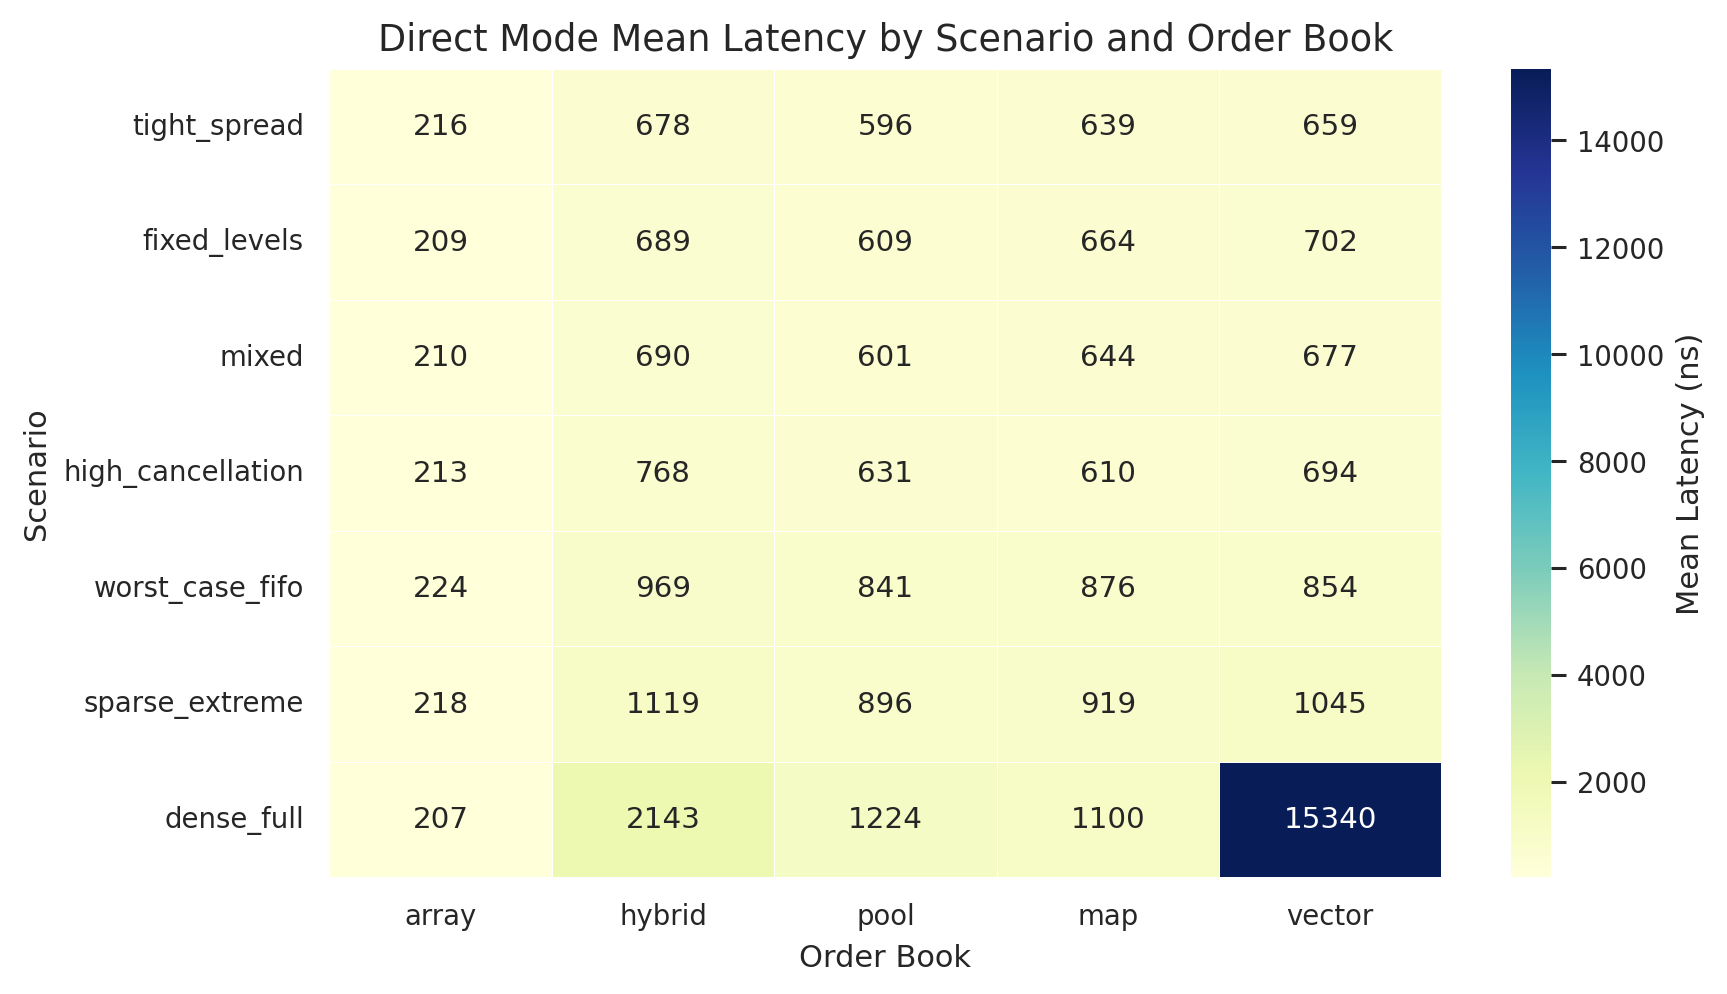
\includegraphics[width=\linewidth]{../plots/direct/latency_mean_heatmap.png}
    \caption[Direct mean latency heatmap]{Direct-mode mean latency heatmap across scenarios and order book implementations. Under this benchmark configuration, array is the fastest implementation in six of seven scenarios, while hybrid is narrowly fastest in tight\_spread.}
    \label{fig:direct-latency-mean-heatmap}
\end{figure}

\begin{figure}[htbp]
    \centering
    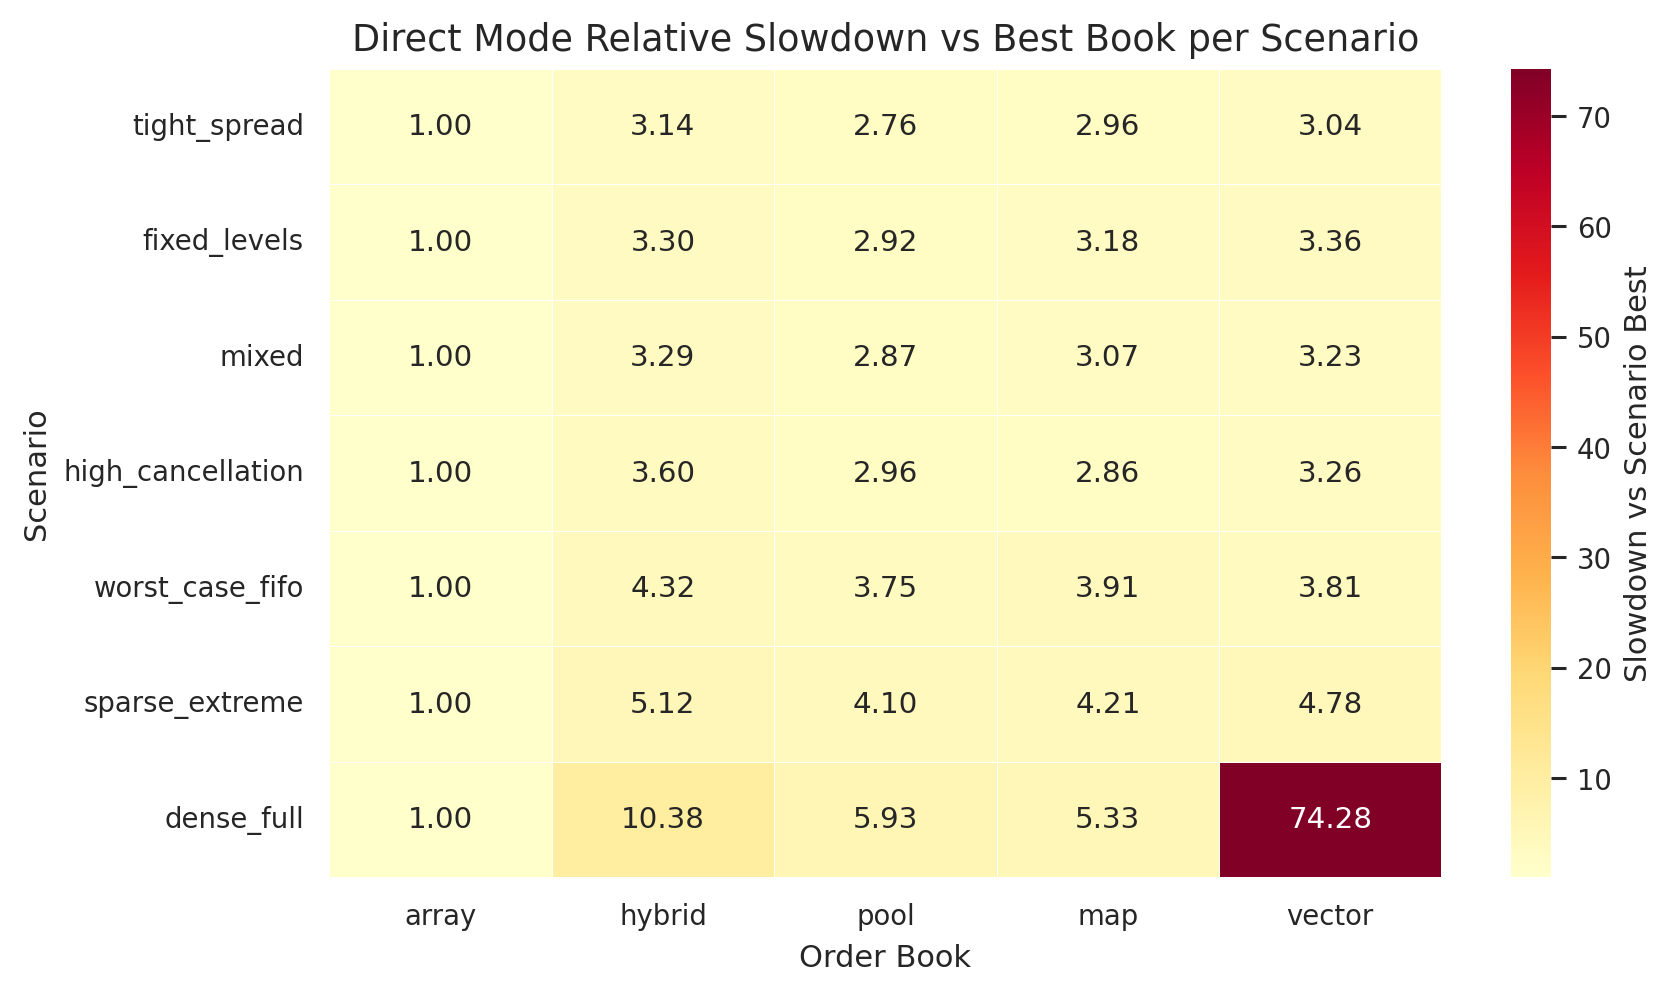
\includegraphics[width=\linewidth]{../plots/direct/latency_slowdown_vs_best_heatmap.png}
    \caption[Direct slowdown versus best]{Direct-mode slowdown relative to the scenario winner. The dense\_full workload shows pronounced vector degradation: vector reaches 16,082.10 ns versus 213.44 ns for the best implementation (approximately 75.3x slowdown).}
    \label{fig:direct-slowdown-vs-best}
\end{figure}

\begin{figure}[htbp]
    \centering
    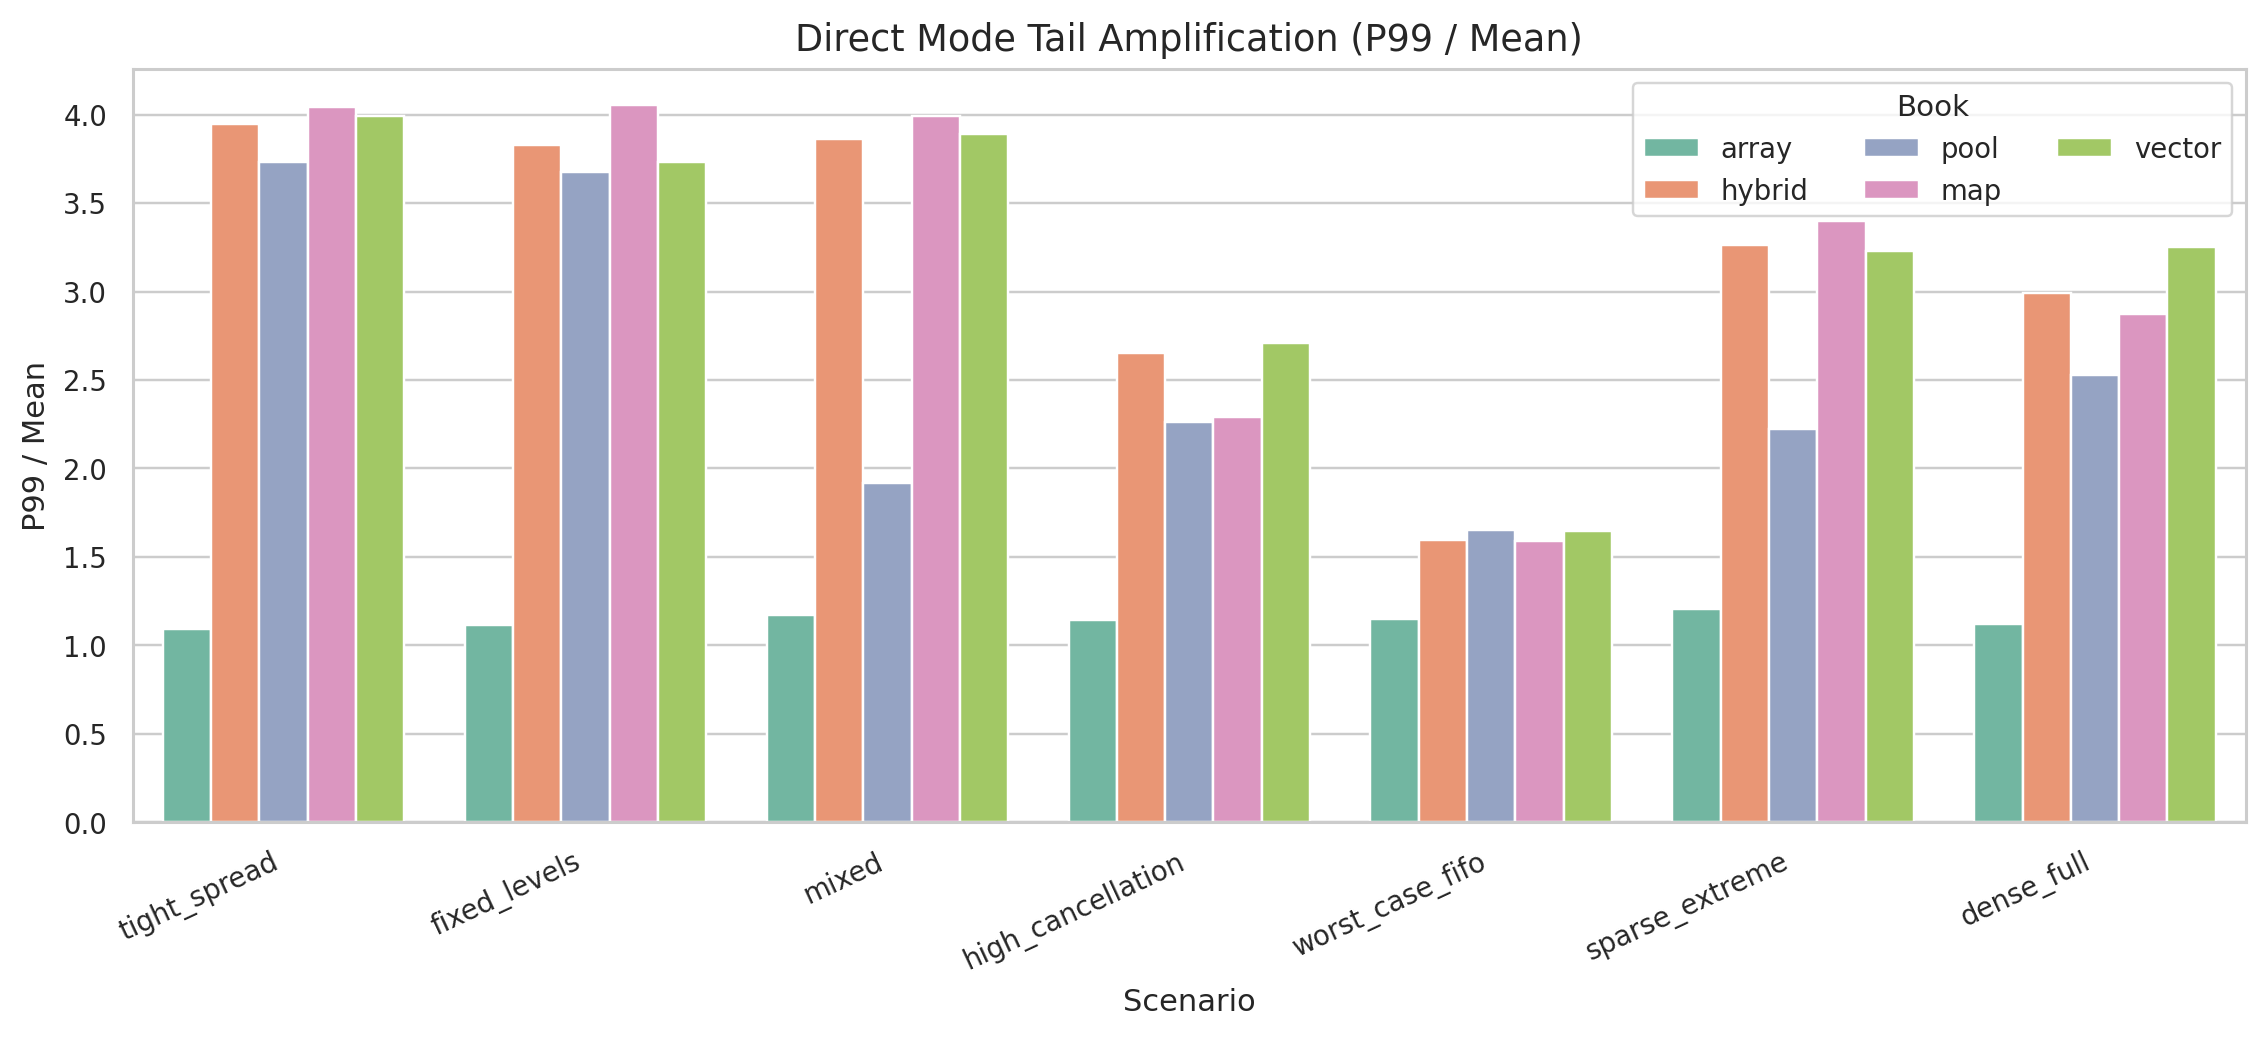
\includegraphics[width=\linewidth]{../plots/direct/tail_p99_over_mean.png}
    \caption[Direct tail inflation]{P99-to-mean tail inflation in direct mode. Several map and vector configurations exhibit elevated tail amplification, indicating greater sensitivity to jitter or burst effects than low-ratio configurations.}
    \label{fig:direct-tail-p99-over-mean}
\end{figure}

\begin{figure}[htbp]
    \centering
    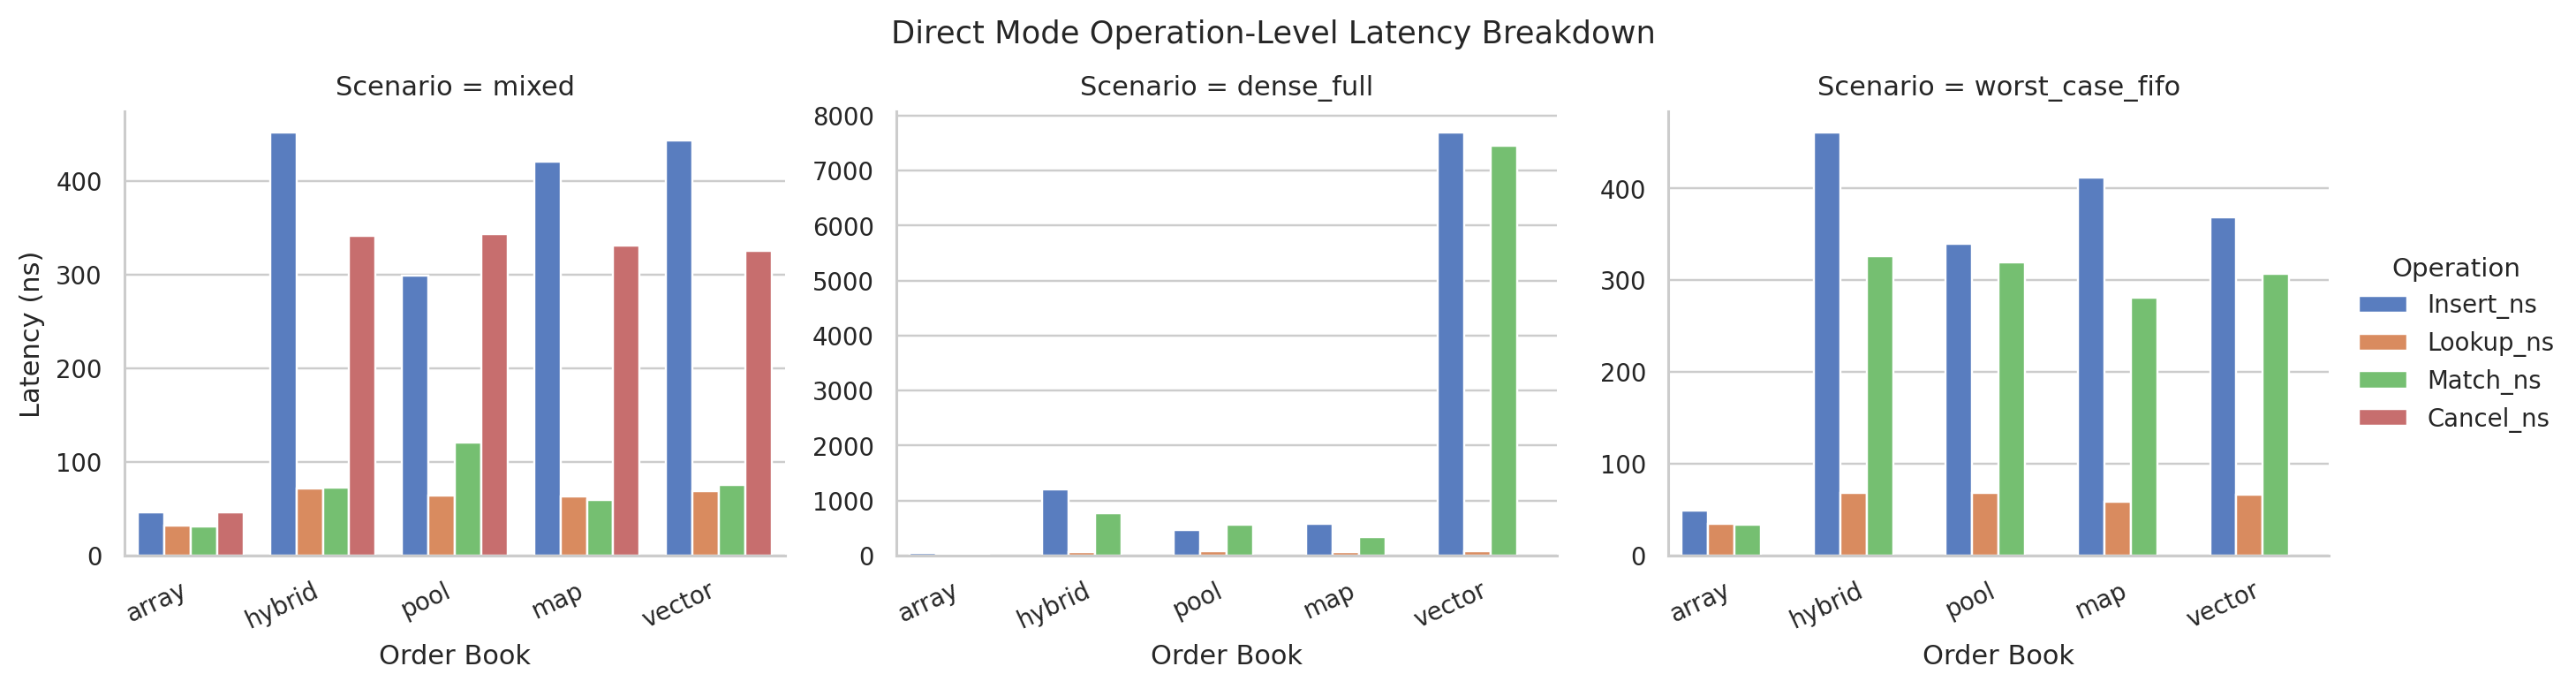
\includegraphics[width=\linewidth]{../plots/direct/operation_latency_breakdown_selected_scenarios.png}
    \caption[Direct operation decomposition]{Per-operation direct-mode latency breakdown for selected scenarios. Insert and lookup are consistently lowest for array, and cancel advantage is visible in cancellation-active scenarios (for example 44.79 ns for array in high\_cancellation).}
    \label{fig:direct-operation-breakdown}
\end{figure}

\begin{figure}[htbp]
    \centering
    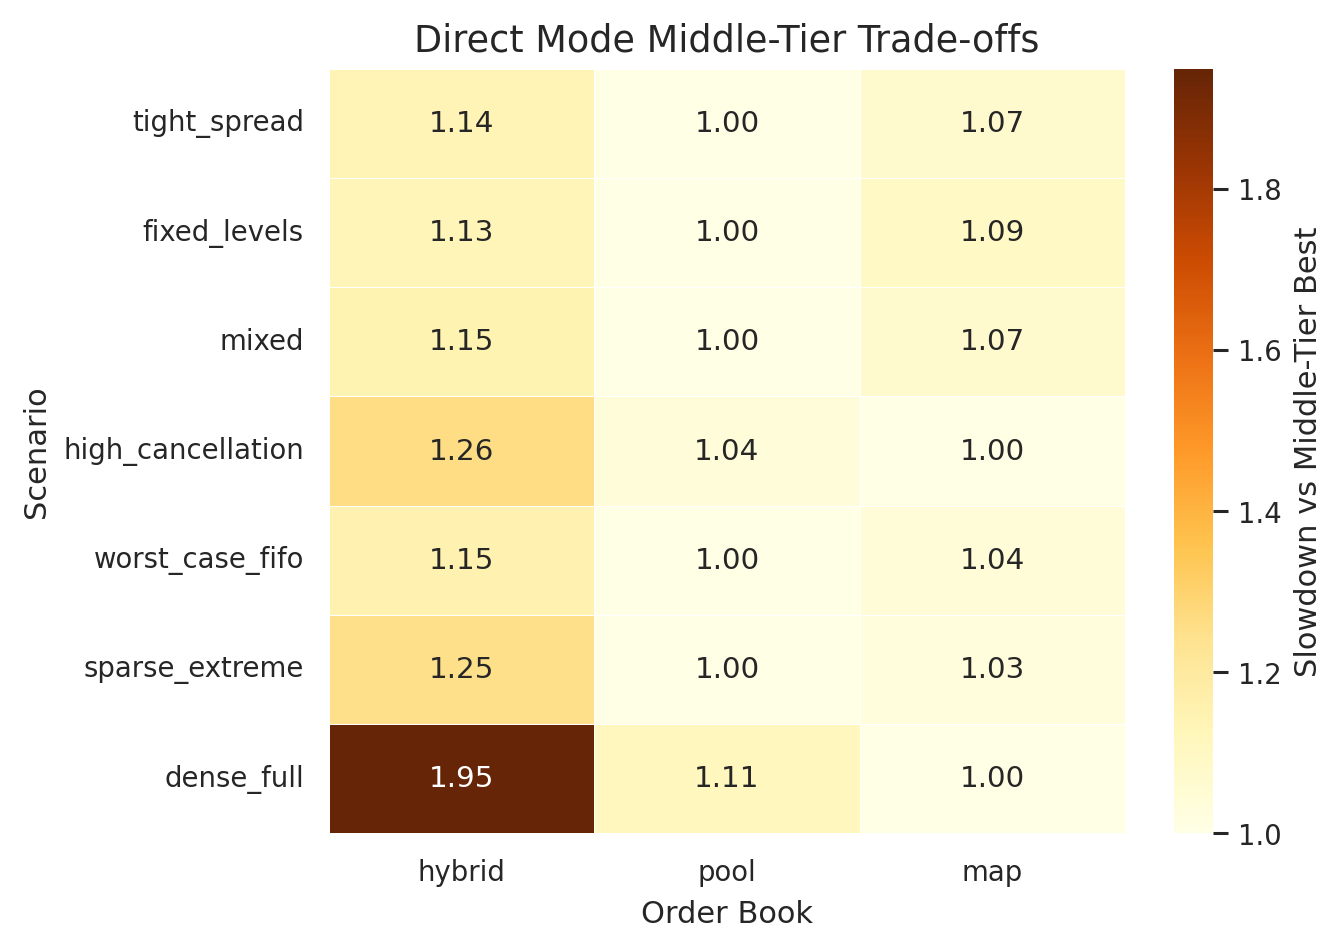
\includegraphics[width=\linewidth]{../plots/direct/middle_tier_slowdown_heatmap.png}
    \caption[Direct middle-tier slowdown]{Relative slowdown among middle-tier implementations (map, hybrid, and pool), normalized to the scenario-best middle-tier implementation. Leadership changes by scenario, supporting a workload-dependent trade-off interpretation.}
    \label{fig:direct-middle-tier-slowdown}
\end{figure}

\begin{figure}[htbp]
    \centering
    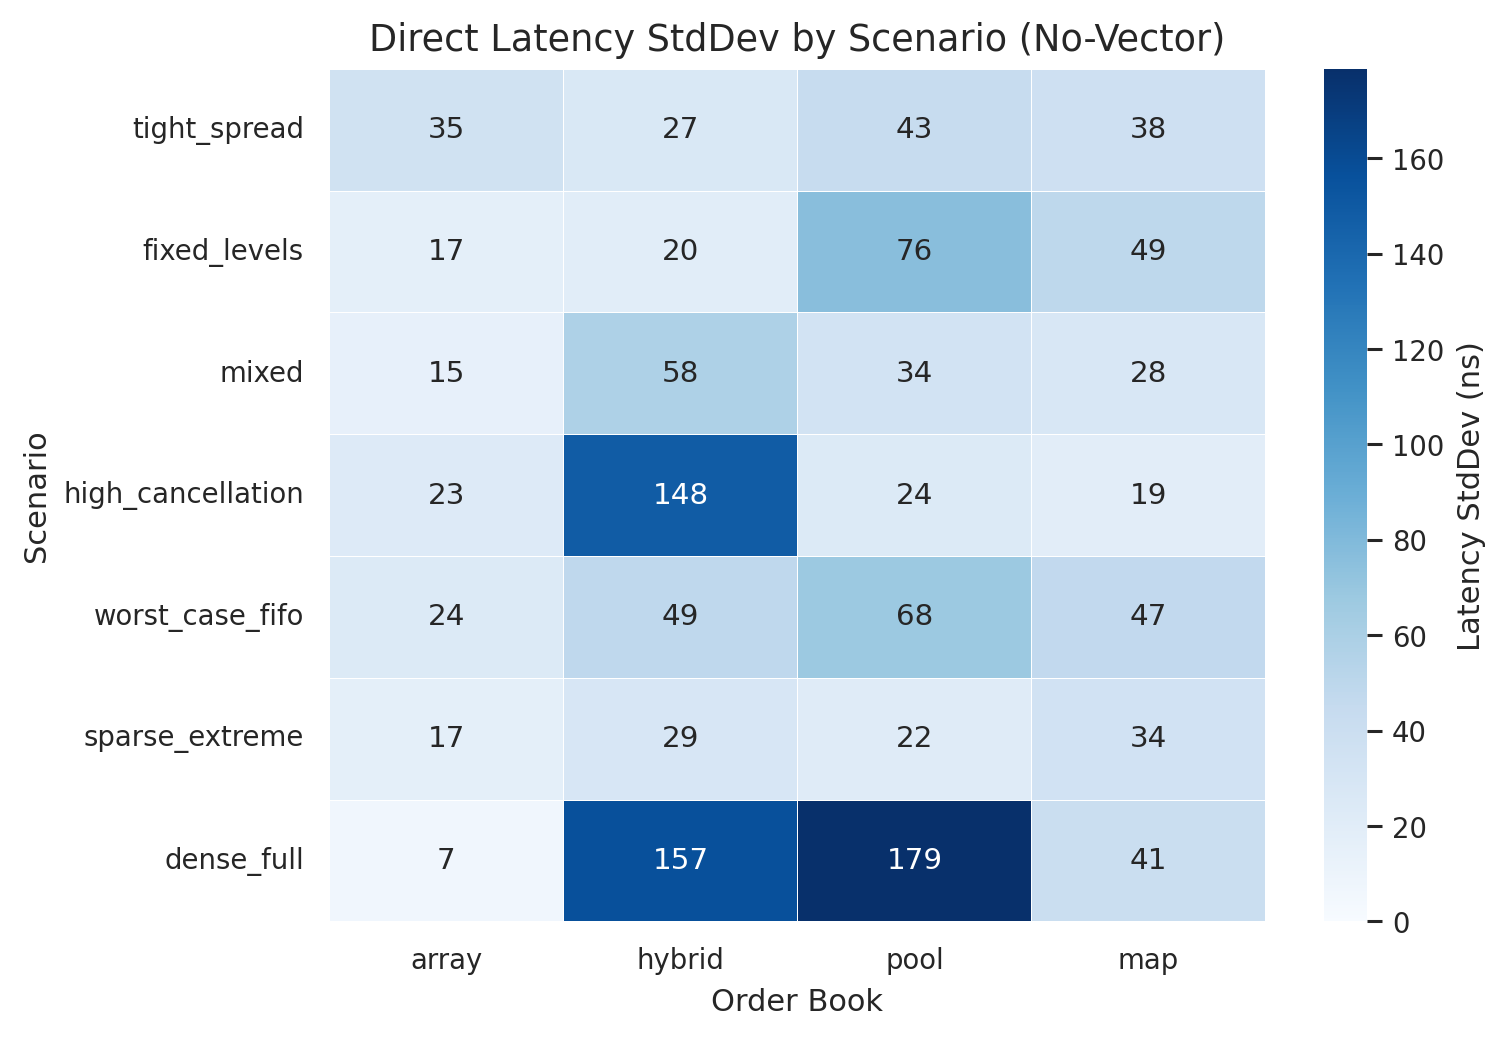
\includegraphics[width=\linewidth]{../plots/direct/latency_stddev_no_vector_heatmap.png}
    \caption[Direct latency variability]{Direct-mode standard deviation heatmap with vector excluded to improve comparative readability. Variability remains scenario dependent, so small mean differences should be interpreted conservatively in high-variance cells.}
    \label{fig:direct-stddev-no-vector}
\end{figure}

\begin{figure}[htbp]
    \centering
    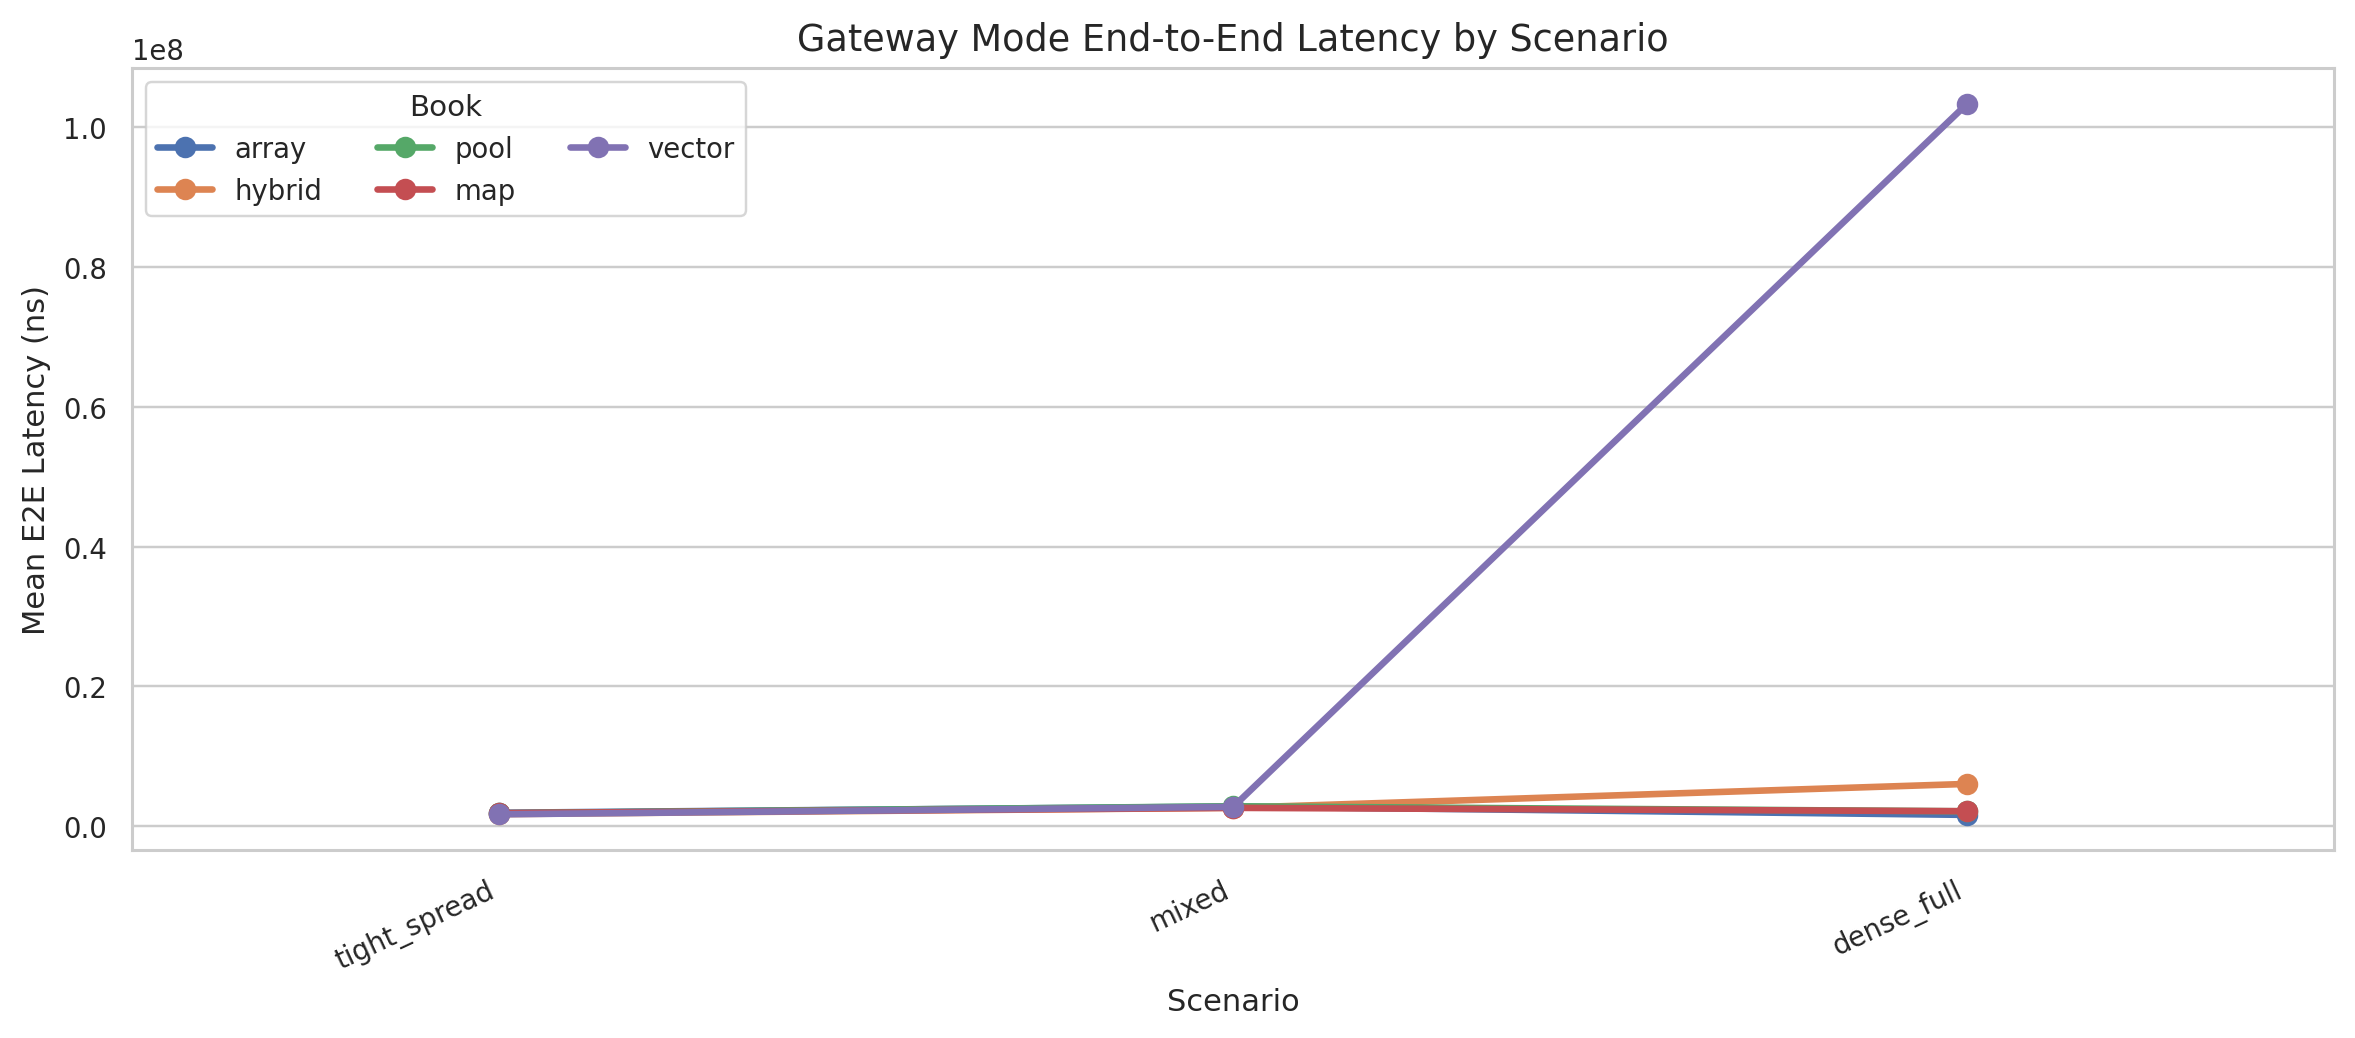
\includegraphics[width=\linewidth]{../plots/gateway/latency_by_scenario.png}
    \caption[Gateway latency by scenario]{Gateway end-to-end mean latency by scenario and implementation. Vector in dense\_full is an extreme outlier (81,741,096.56 ns), consistent with queue-amplification under sustained dense workload pressure.}
    \label{fig:gateway-latency-by-scenario}
\end{figure}

\begin{figure}[htbp]
    \centering
    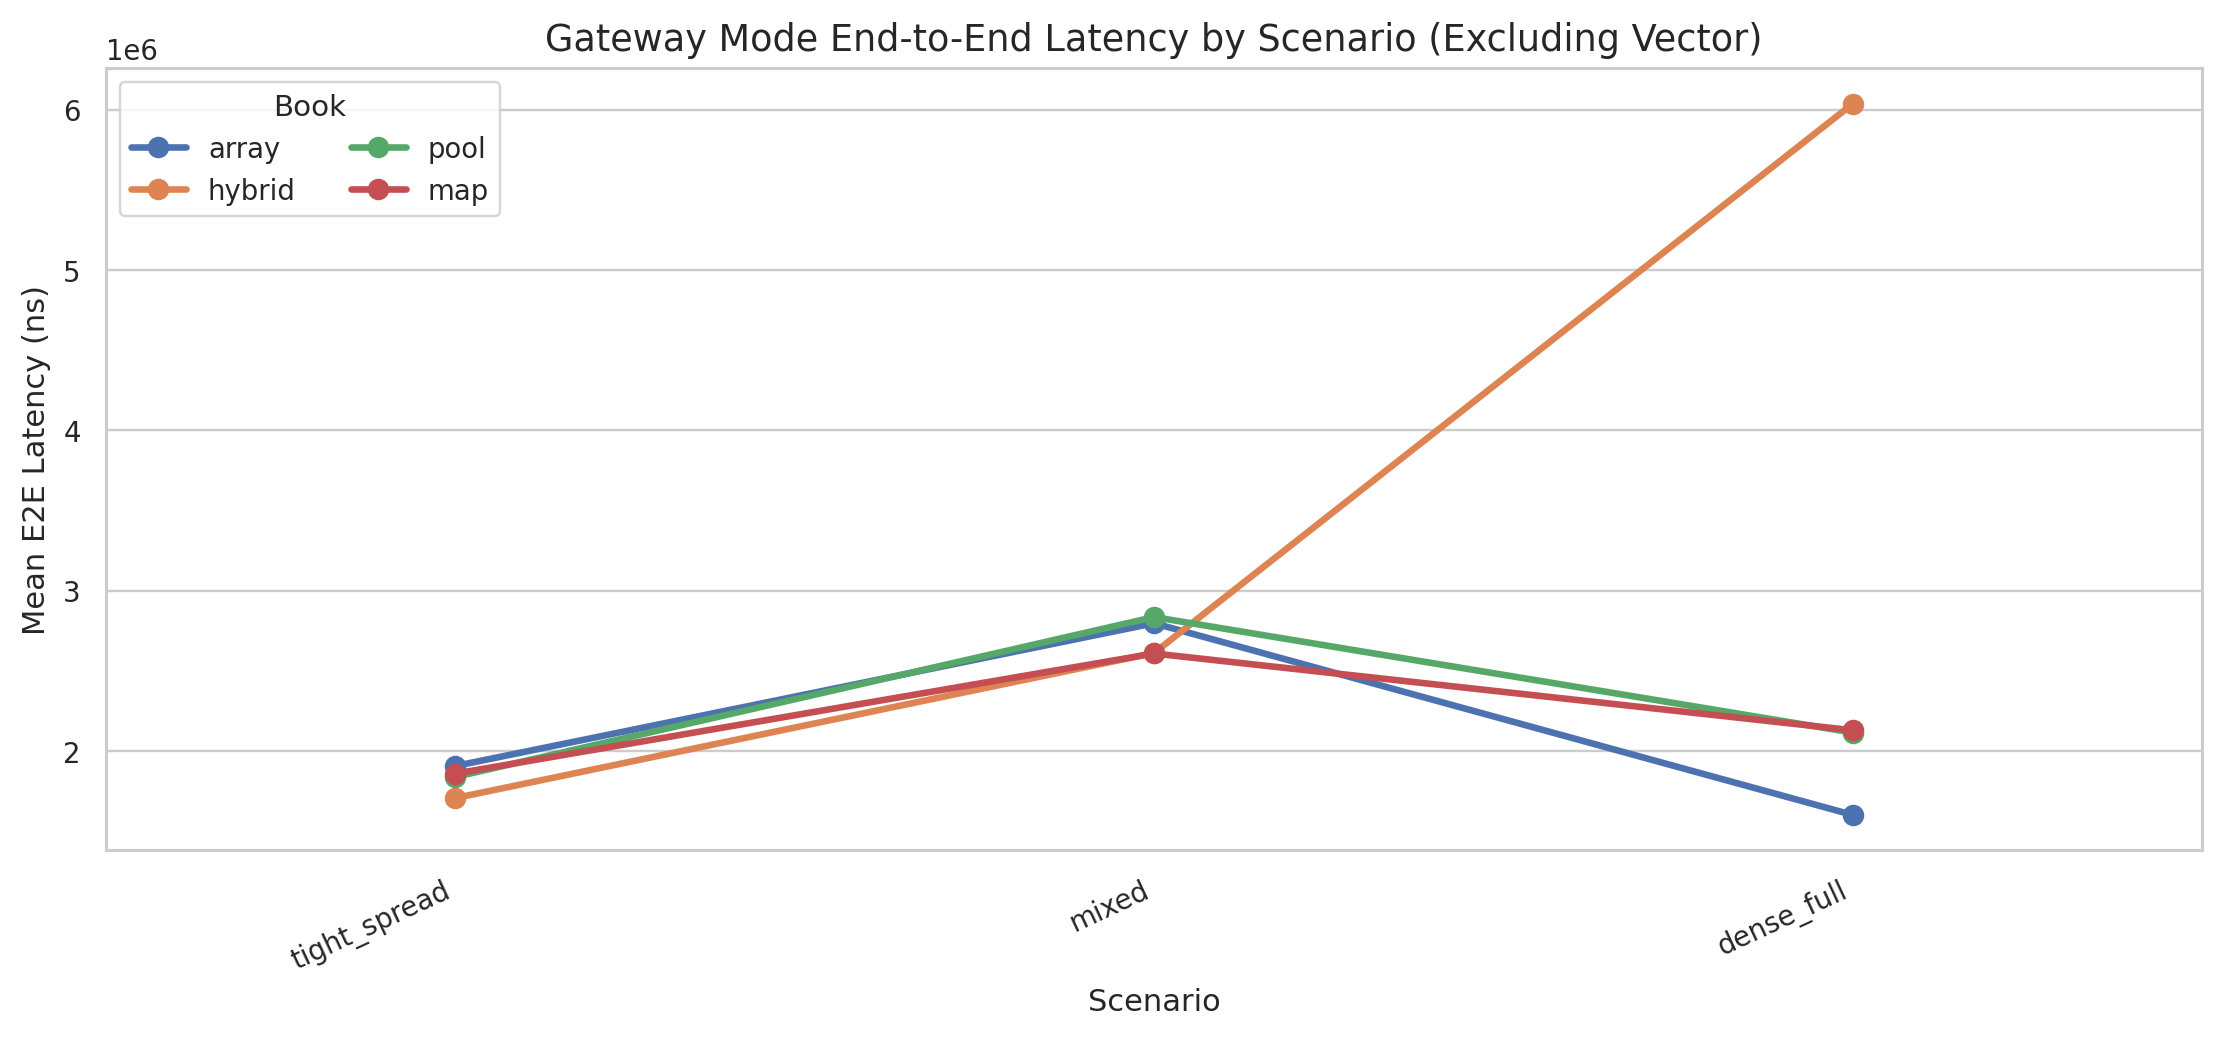
\includegraphics[width=\linewidth]{../plots/gateway/latency_by_scenario_no_vector.png}
    \caption[Gateway latency excluding vector]{Gateway end-to-end latency with vector excluded for readability. No single non-vector implementation dominates all scenarios in this run: pool leads four scenarios, map two, and hybrid one.}
    \label{fig:gateway-latency-no-vector}
\end{figure}

\begin{figure}[htbp]
    \centering
    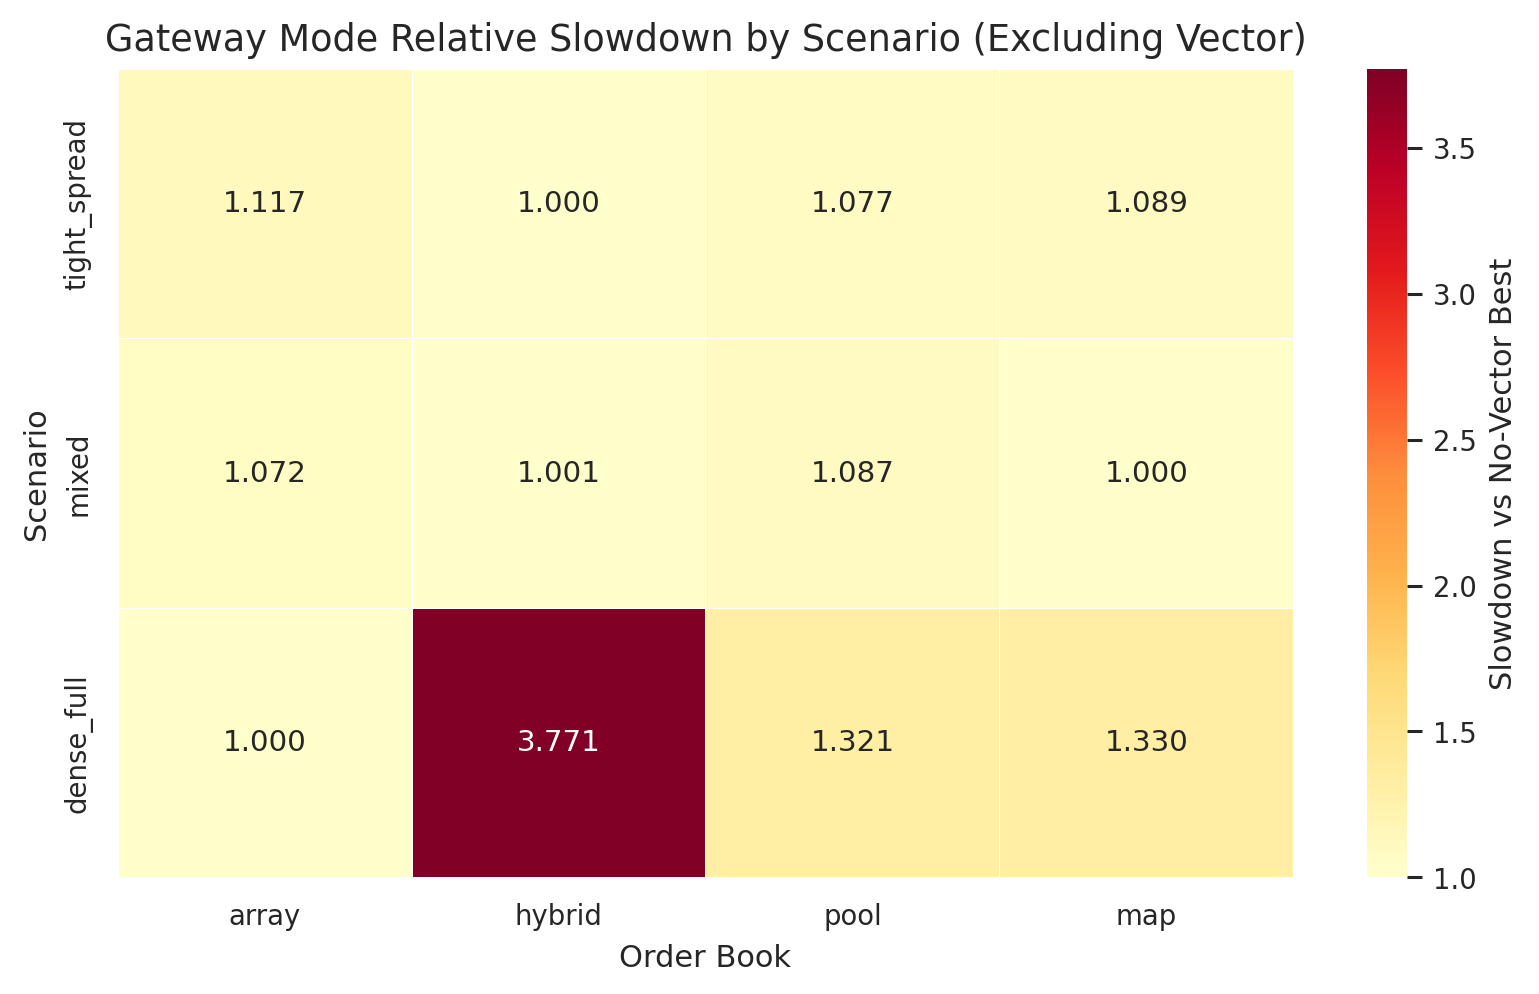
\includegraphics[width=\linewidth]{../plots/gateway/latency_slowdown_no_vector_heatmap.png}
    \caption[Gateway slowdown excluding vector]{Gateway slowdown heatmap with vector excluded and each scenario normalized by its best non-vector implementation. Scenario-specific spread remains material, indicating non-uniform interaction between transport, queueing, and engine effects.}
    \label{fig:gateway-slowdown-no-vector}
\end{figure}

\begin{figure}[htbp]
    \centering
    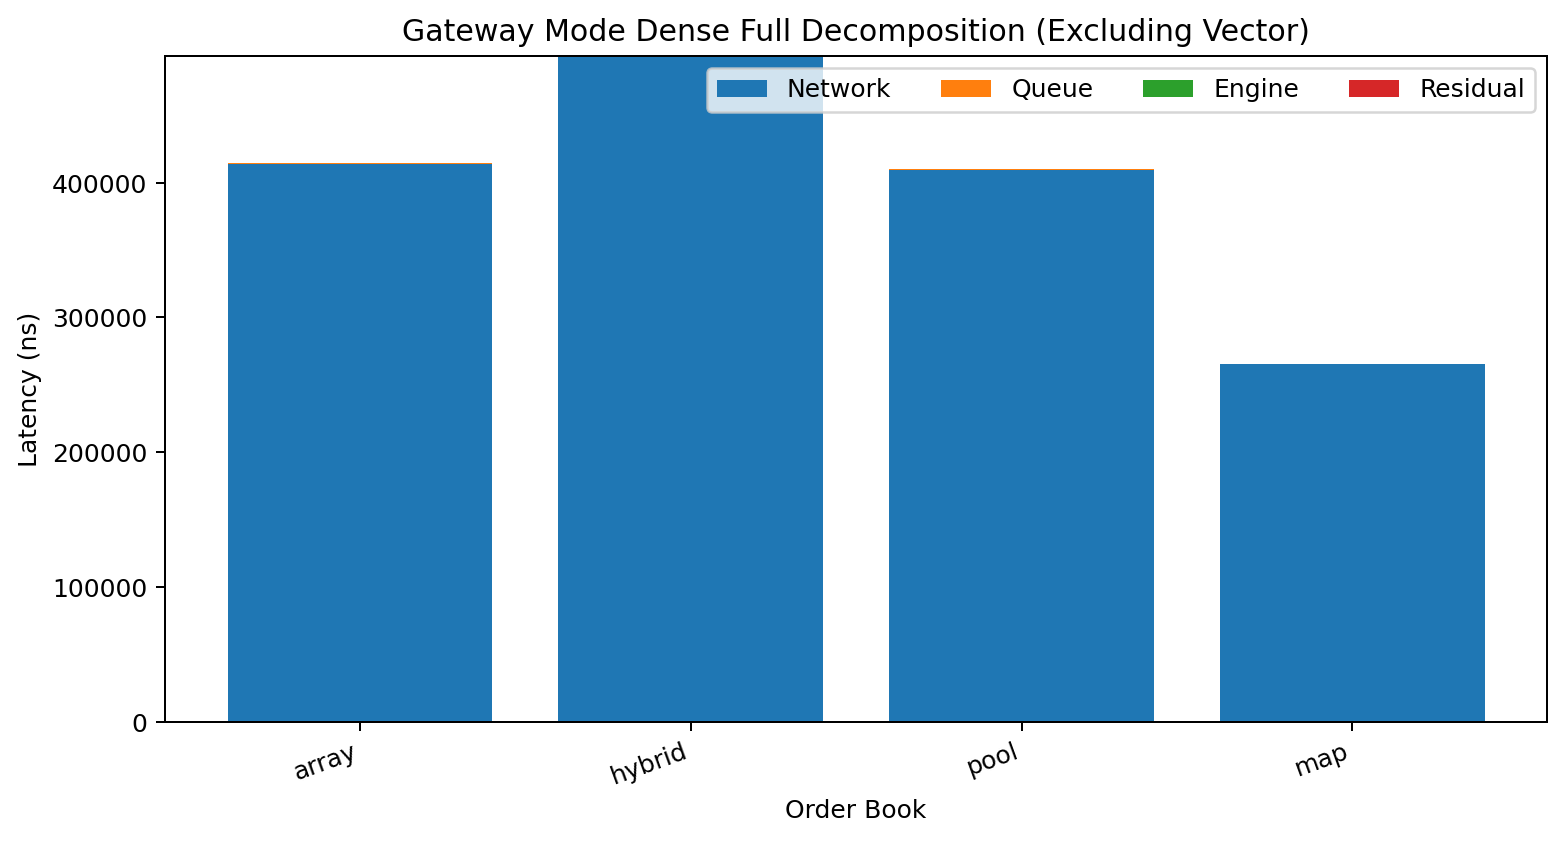
\includegraphics[width=\linewidth]{../plots/gateway/dense_full_latency_decomposition_no_vector.png}
    \caption[Dense full decomposition excluding vector]{Dense\_full gateway decomposition into Network, Queue, and Engine components for non-vector implementations. Queue contribution rises in dense conditions, but Network remains the dominant component for non-vector rows.}
    \label{fig:gateway-dense-decomposition-no-vector}
\end{figure}

\begin{figure}[htbp]
    \centering
    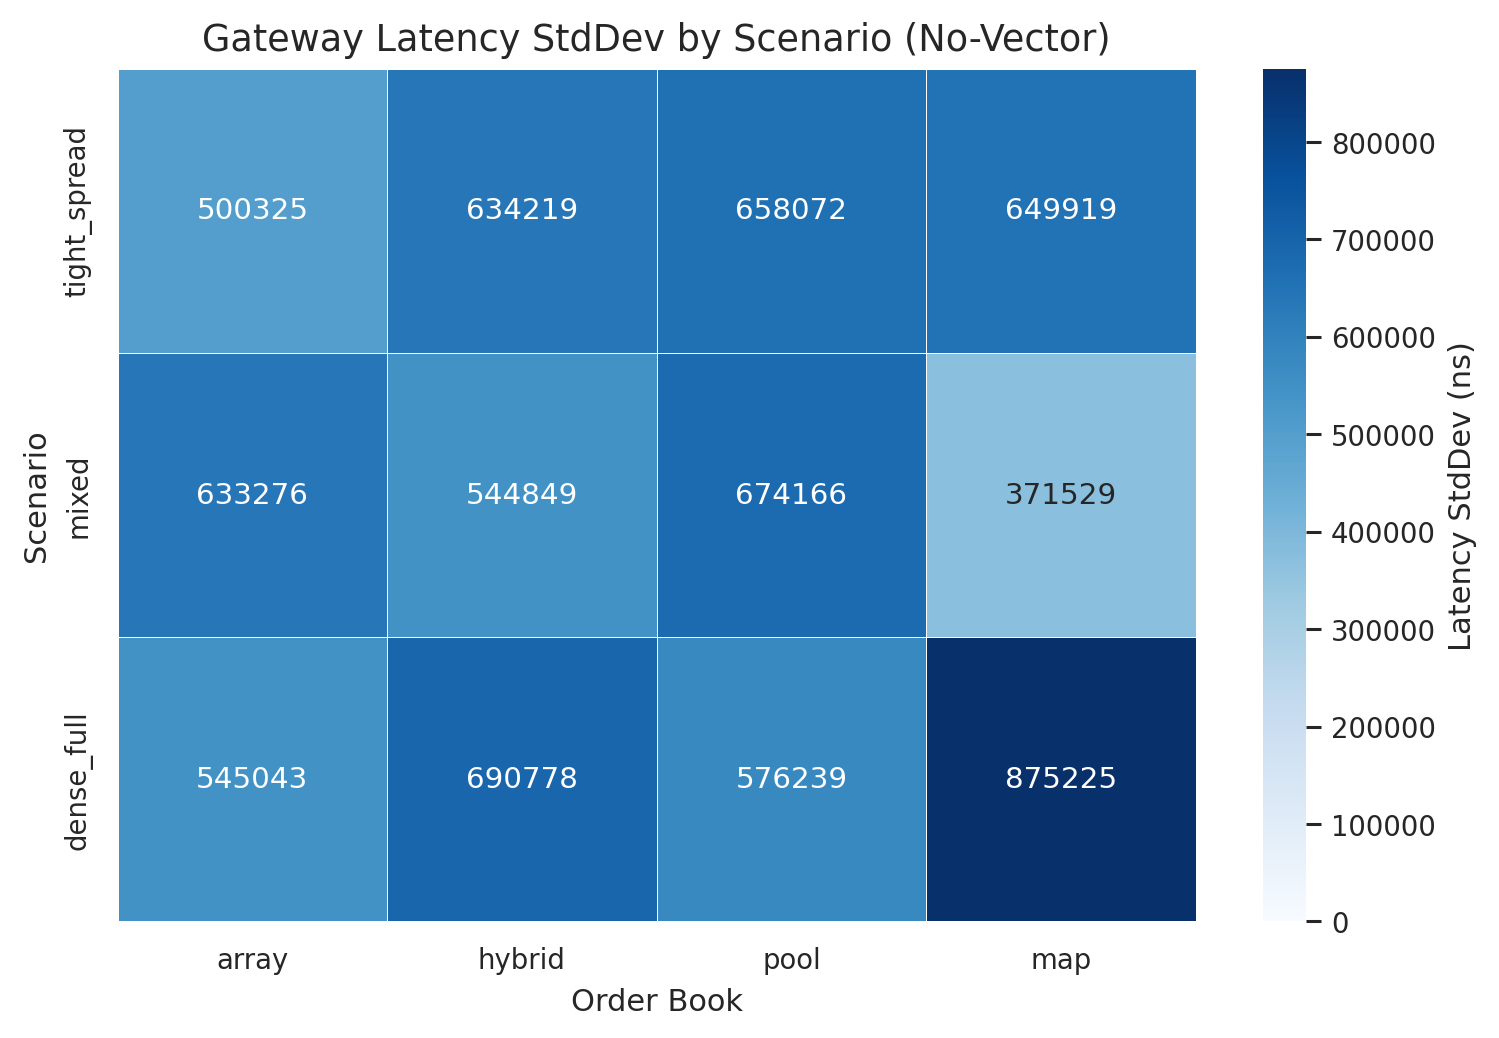
\includegraphics[width=\linewidth]{../plots/gateway/latency_stddev_no_vector_heatmap.png}
    \caption[Gateway variability excluding vector]{Gateway-mode latency standard deviation heatmap with vector excluded. Selected cells retain high coefficient of variation, so close mean values should not be over-interpreted without additional repeated-run confidence intervals.}
    \label{fig:gateway-stddev-no-vector}
\end{figure}

\begin{figure}[htbp]
    \centering
    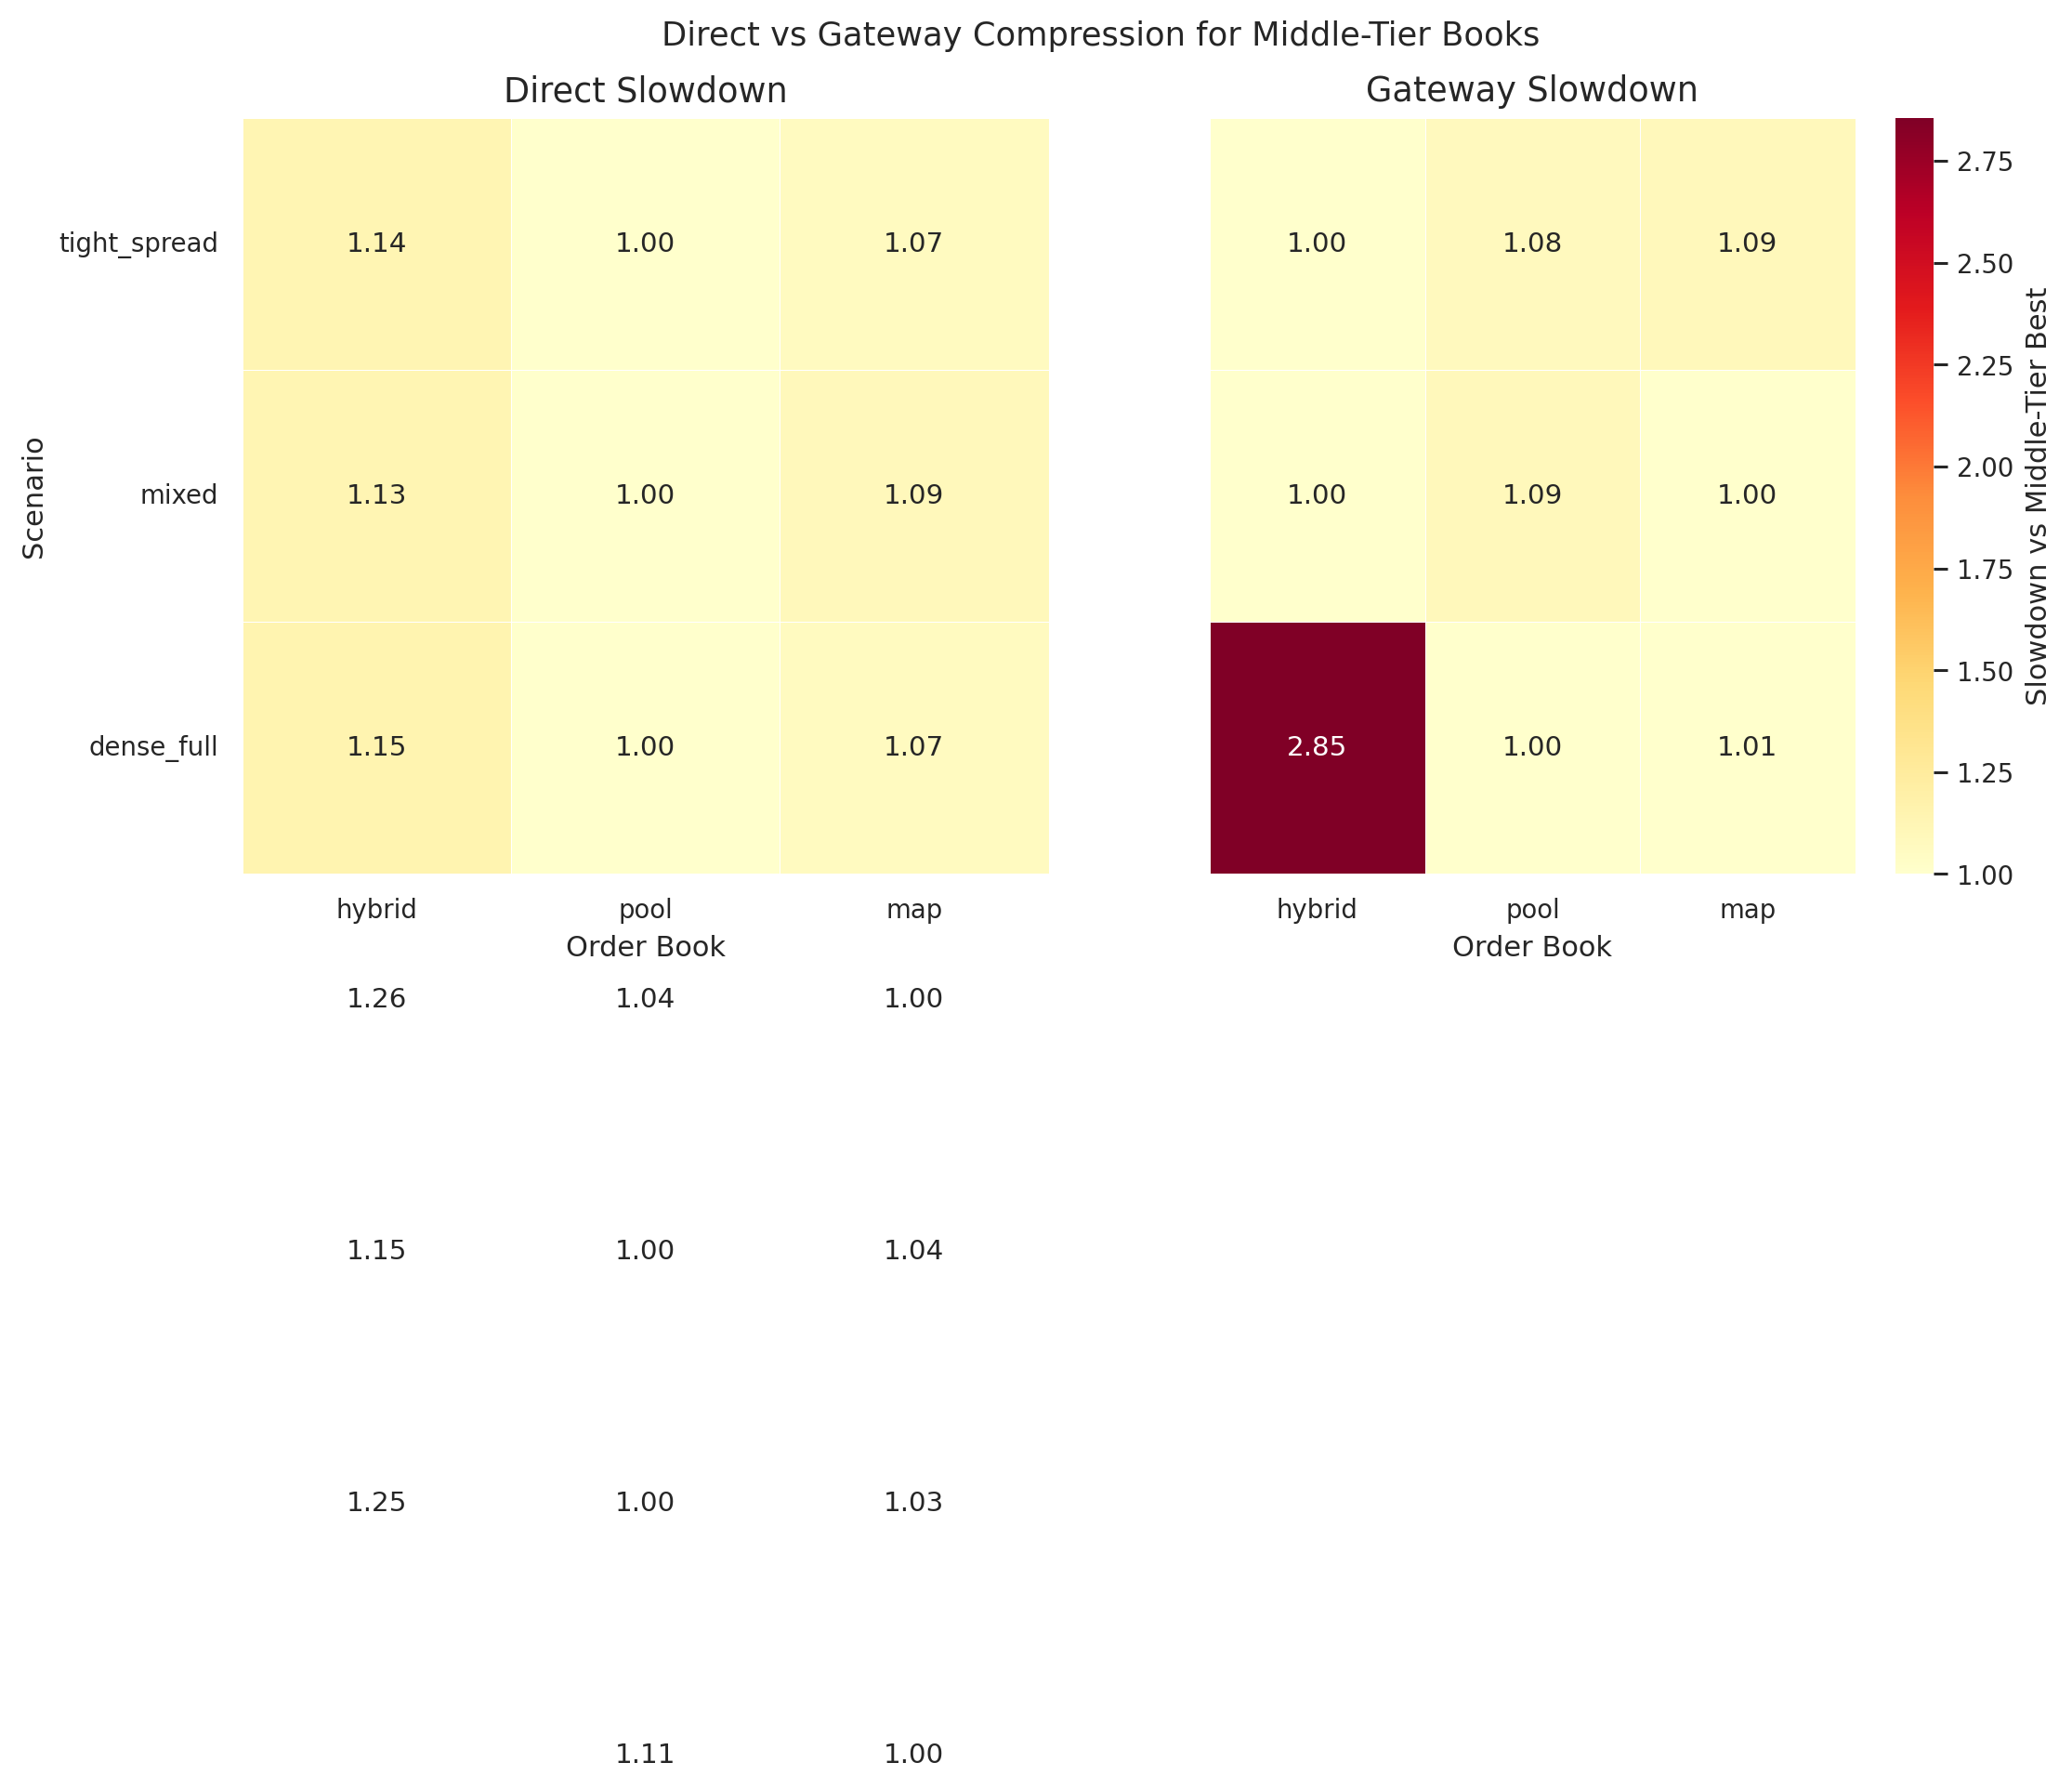
\includegraphics[width=\linewidth]{../plots/direct_vs_gateway/middle_tier_slowdown_direct_vs_gateway.png}
    \caption[Direct vs gateway middle-tier comparison]{Middle-tier slowdown comparison between direct and gateway modes. Direct mode preserves clearer algorithmic separation, while gateway mode compresses many differences because transport cost dominates in most non-outlier cases.}
    \label{fig:direct-vs-gateway-middle-tier}
\end{figure}

\begin{figure}[htbp]
    \centering
    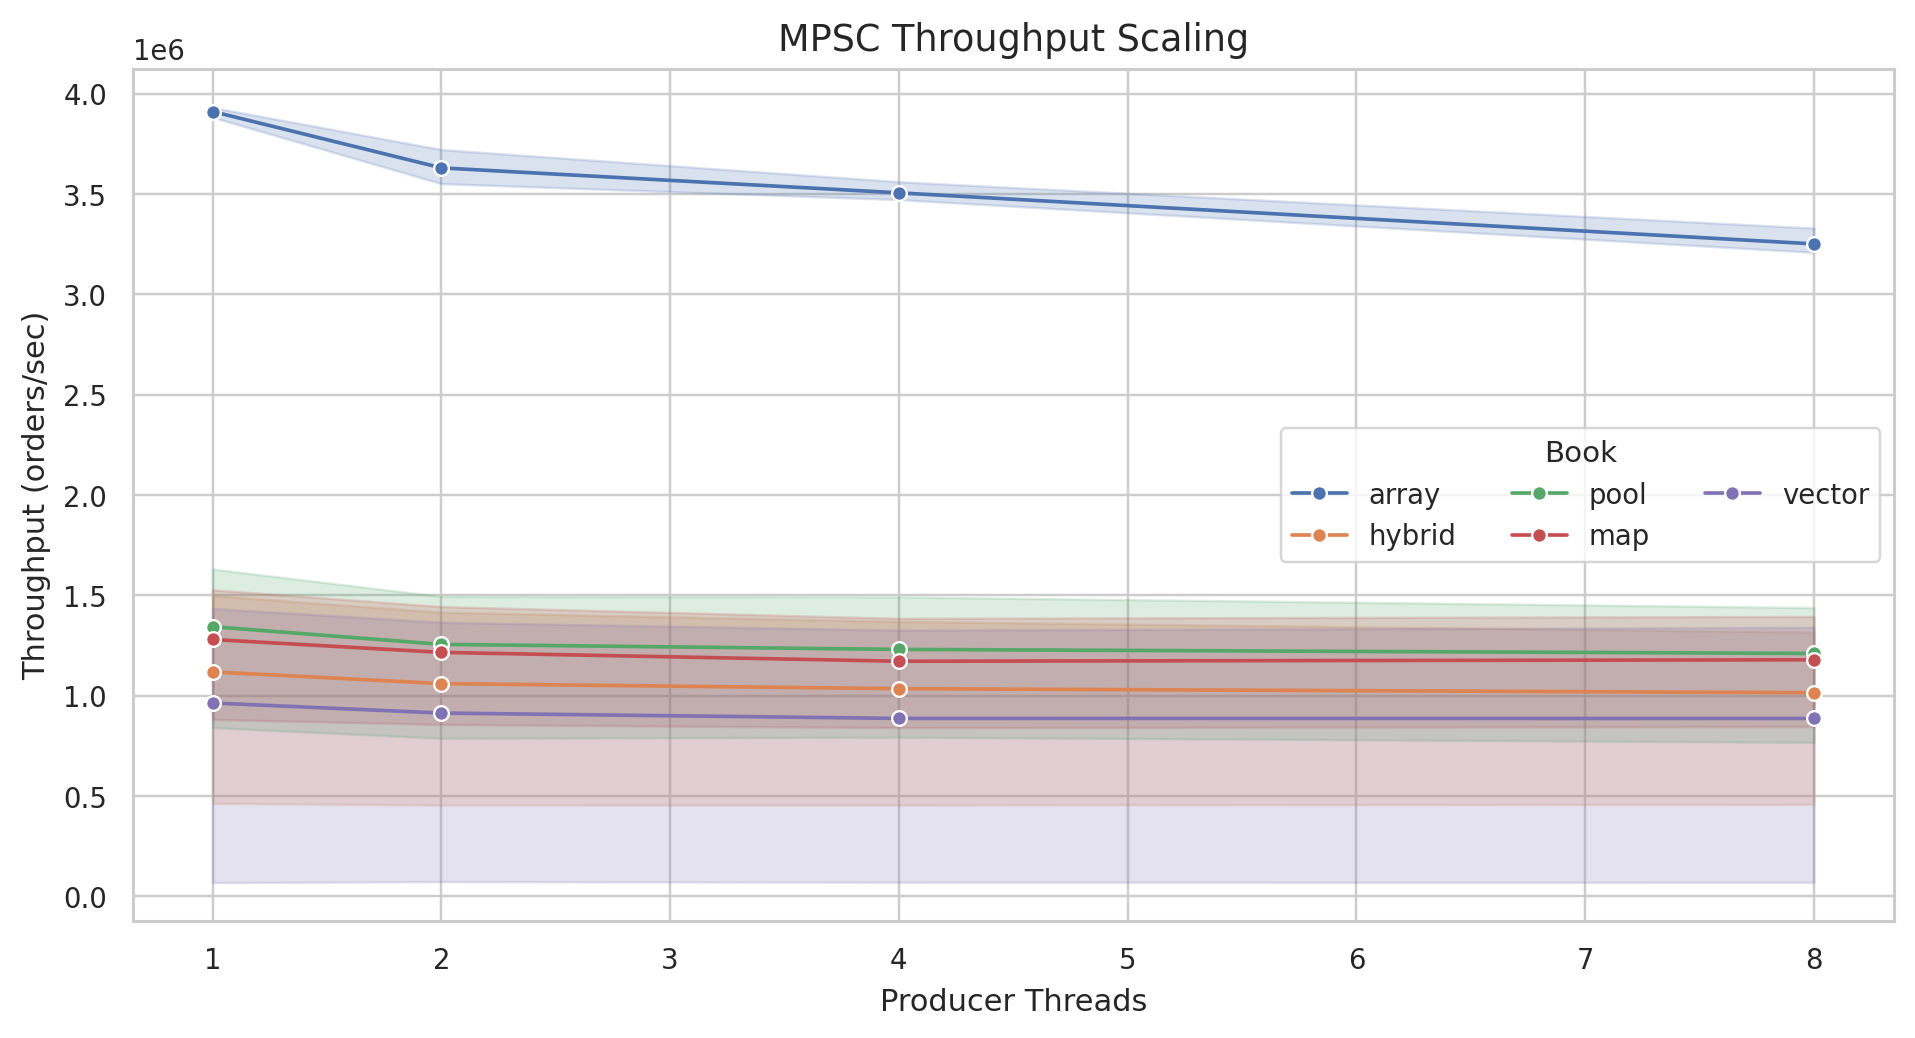
\includegraphics[width=\linewidth]{../plots/mpsc/throughput_scaling.png}
    \caption[MPSC throughput scaling]{MPSC throughput scaling across producer counts and implementations. Relative throughput hierarchy remains implementation dependent, with array in the highest tier and vector substantially lower in dense scenarios.}
    \label{fig:mpsc-throughput-scaling}
\end{figure}

\begin{figure}[htbp]
    \centering
    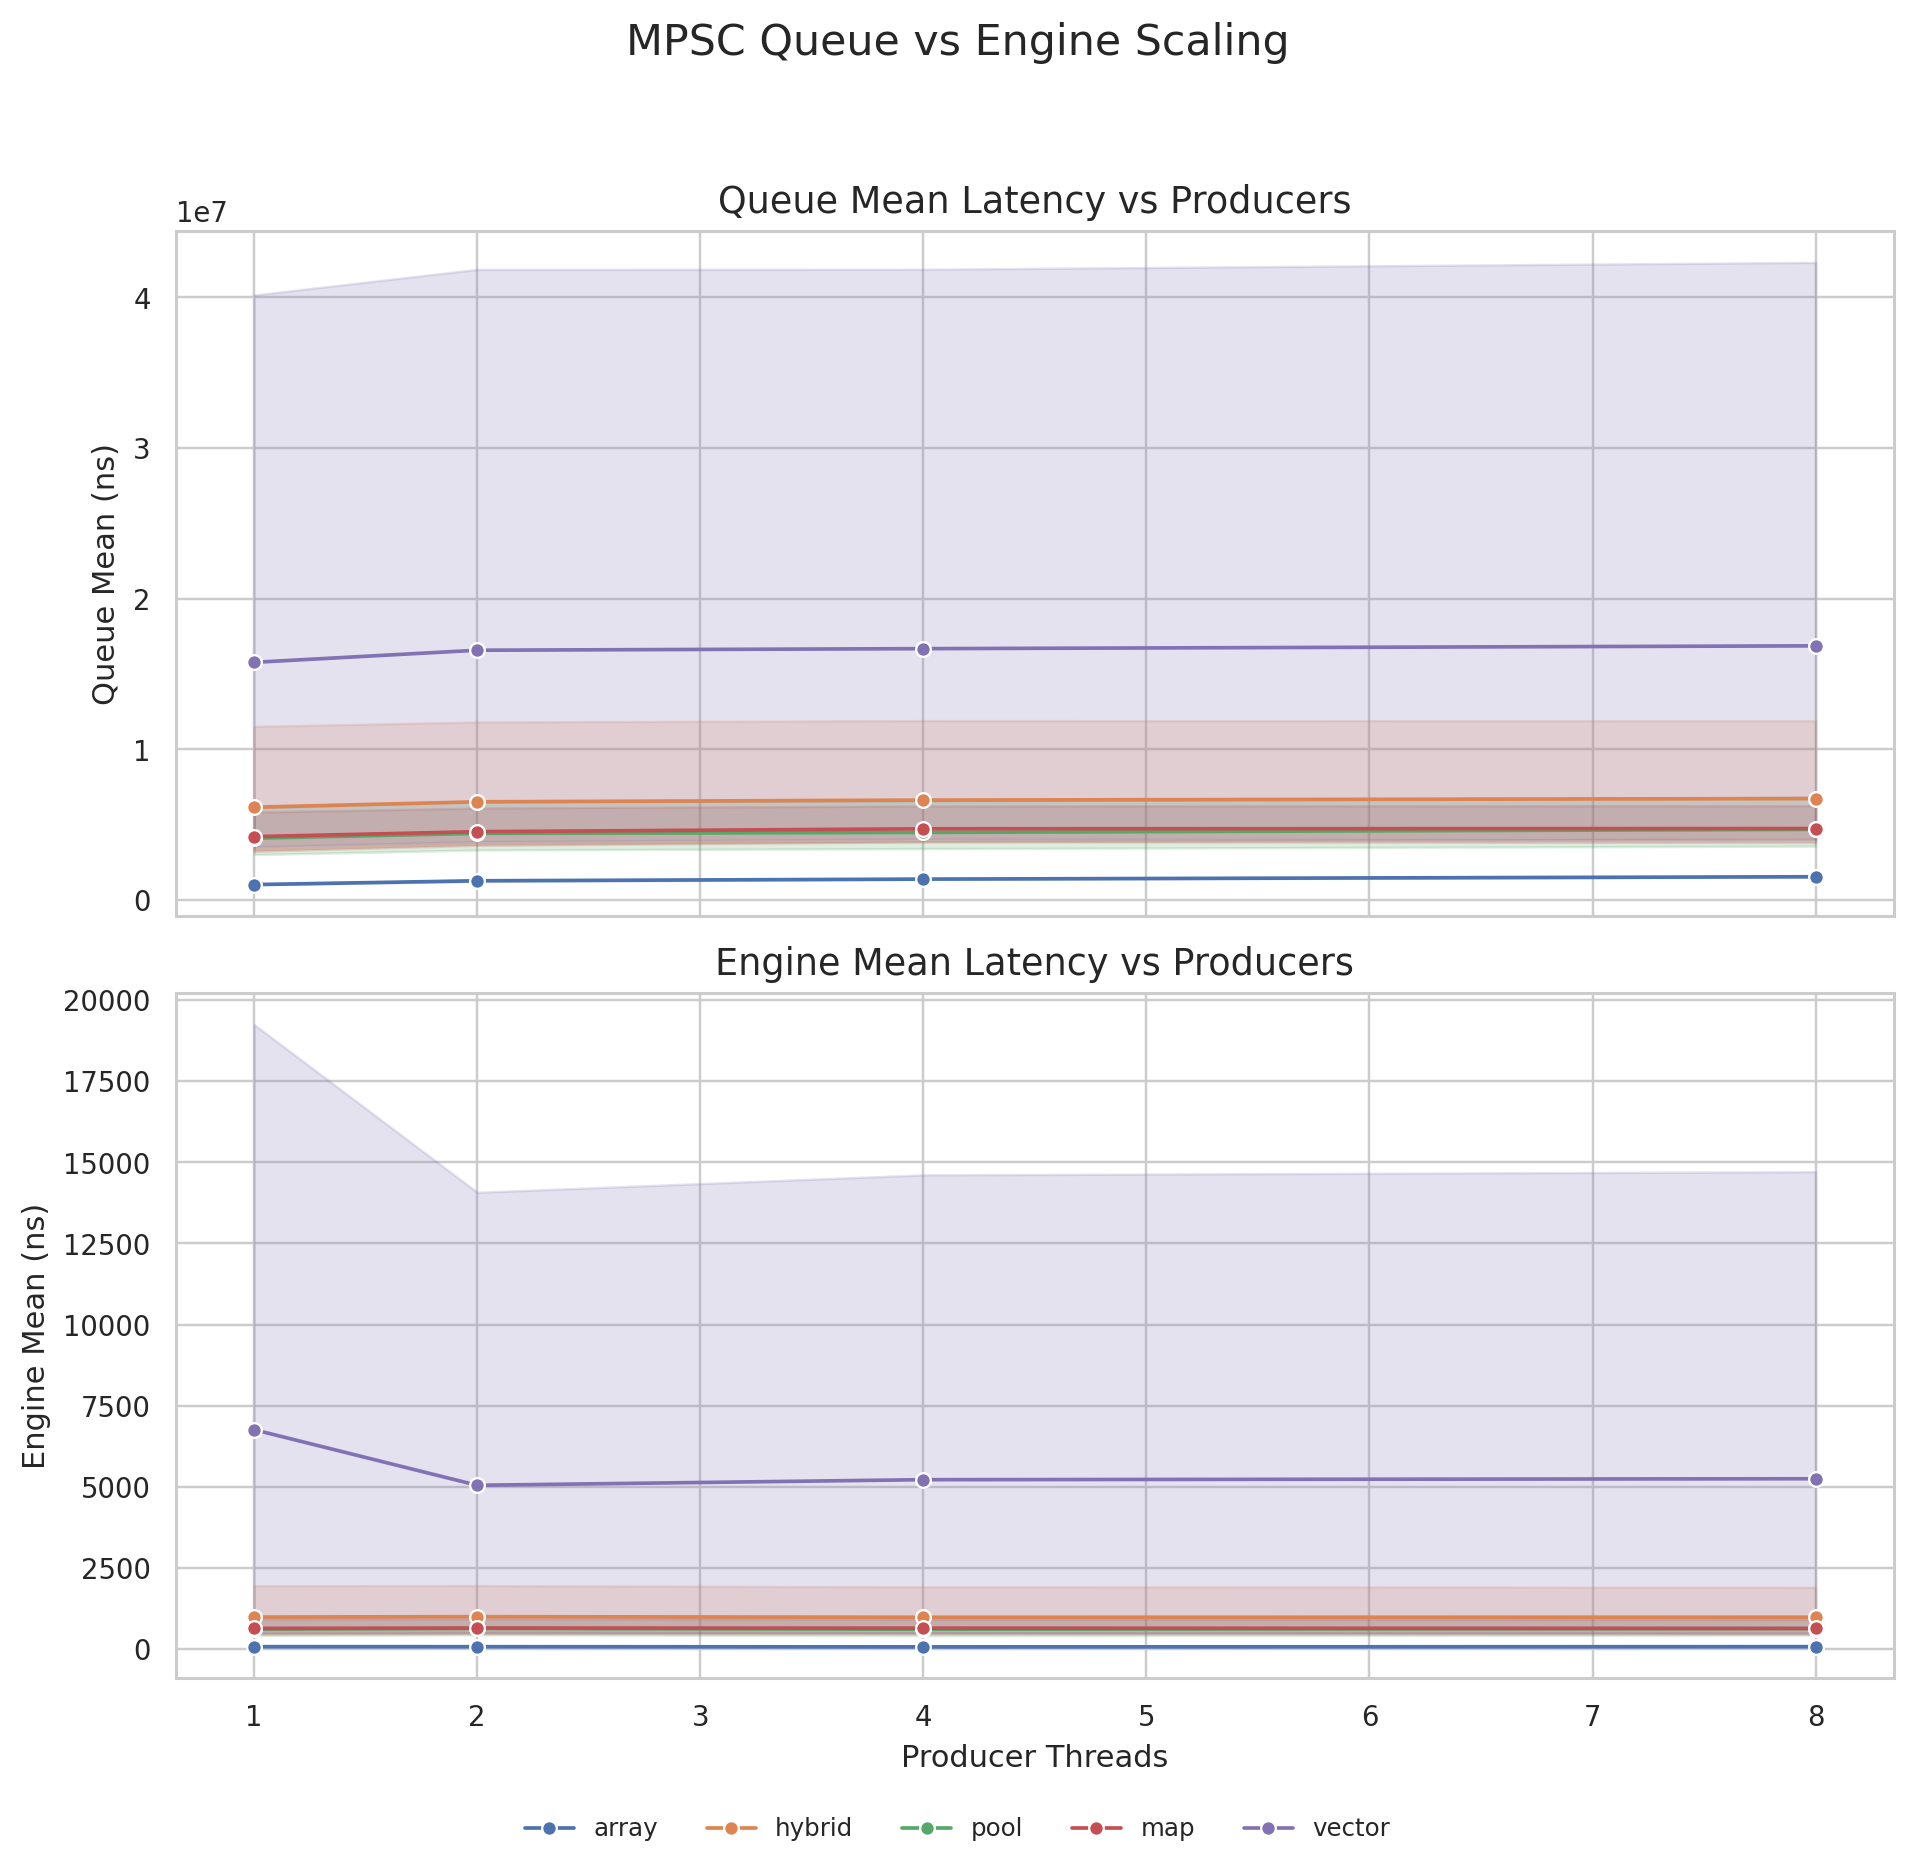
\includegraphics[width=\linewidth]{../plots/mpsc/queue_vs_engine_scaling.png}
    \caption[MPSC queue versus engine scaling]{MPSC queue-latency versus engine-latency scaling across producer counts. Engine latency is stable in many book/scenario pairs, while queue latency captures contention and burst-pressure effects.}
    \label{fig:mpsc-queue-vs-engine}
\end{figure}

\begin{figure}[htbp]
    \centering
    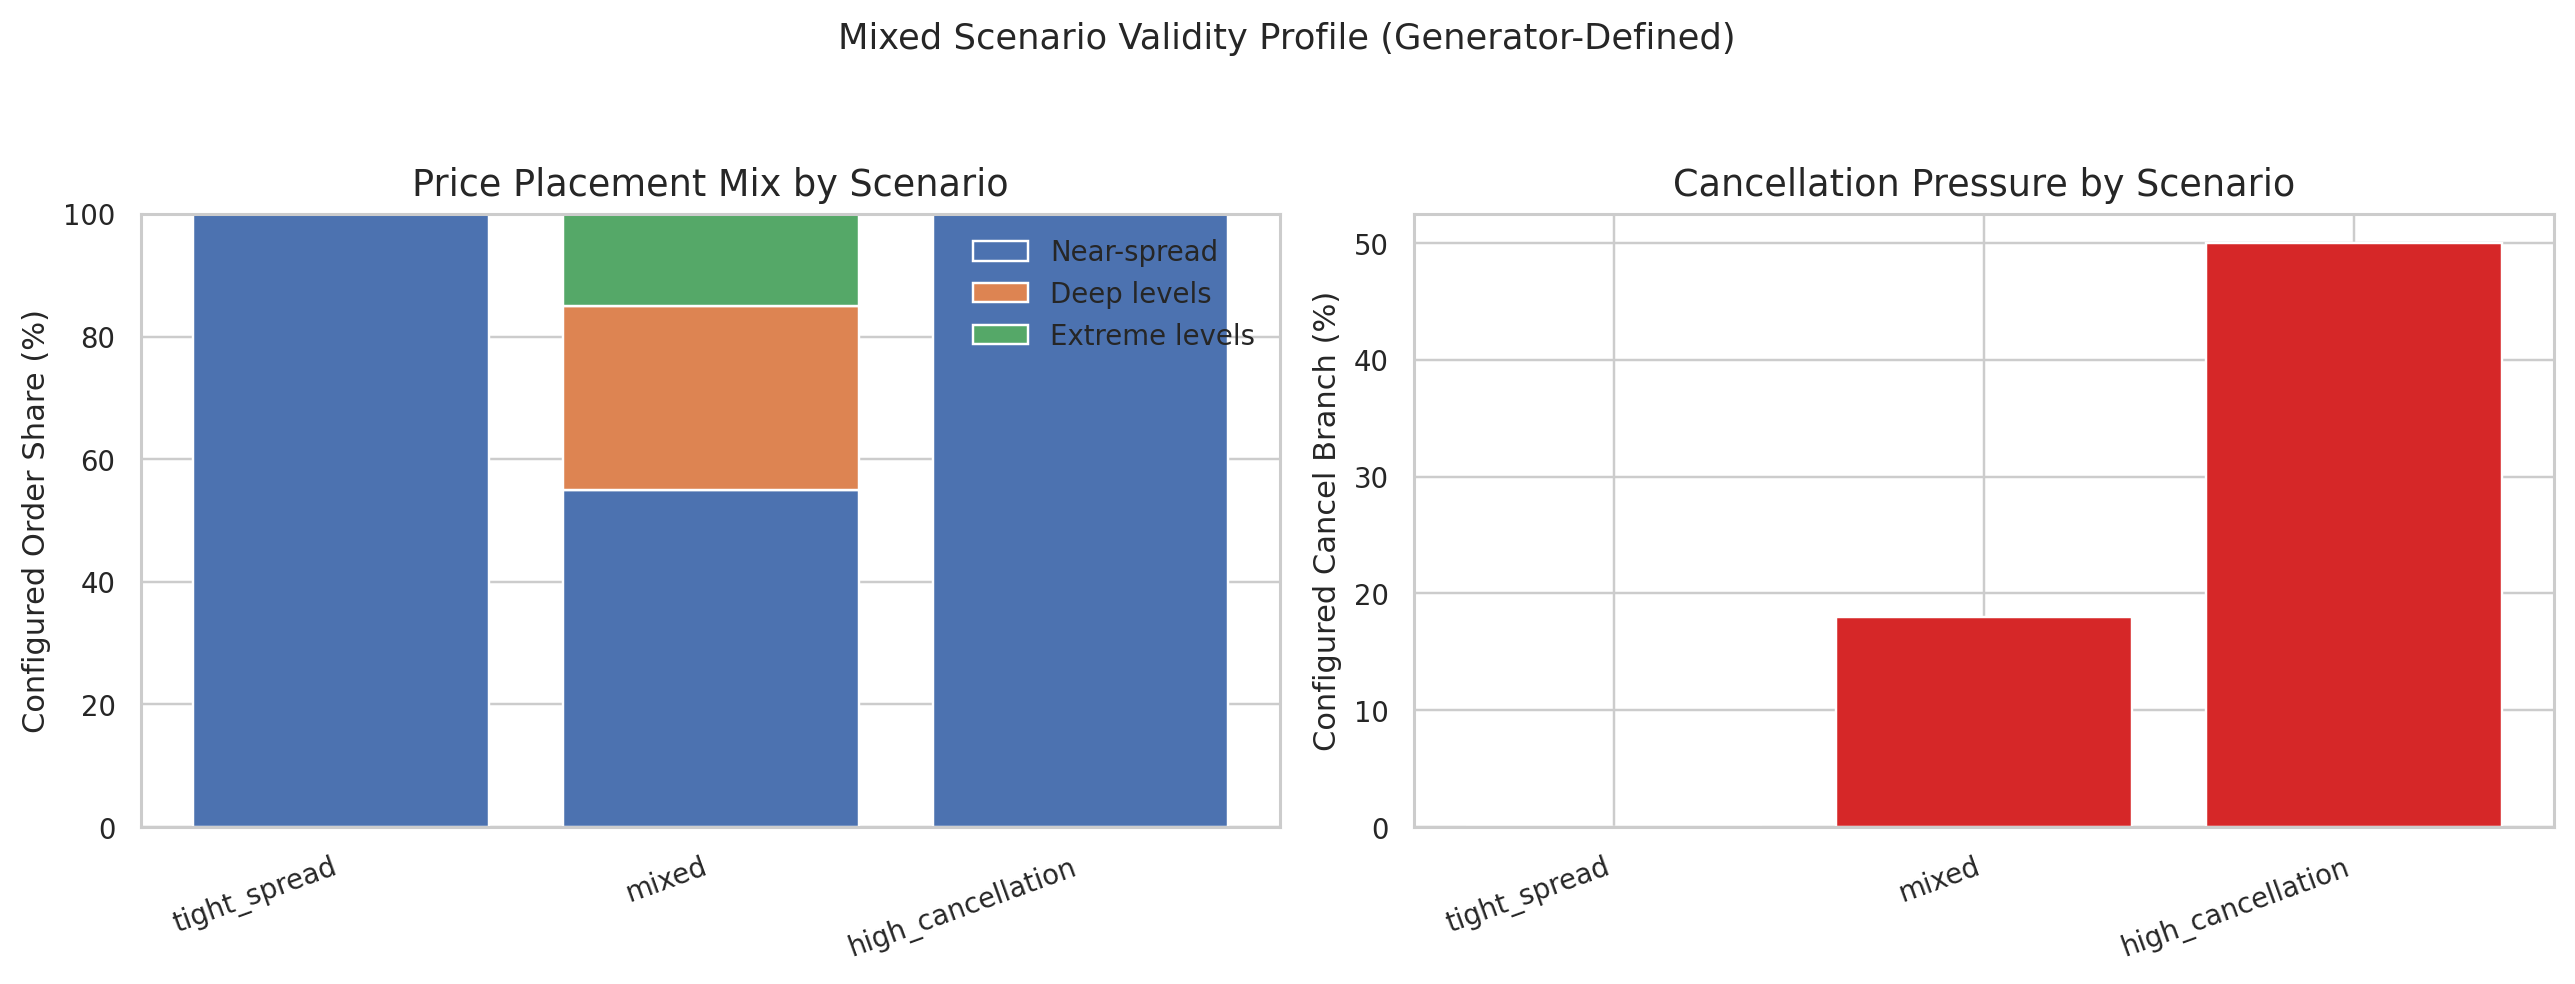
\includegraphics[width=\linewidth]{../plots/scenario_validity/mixed_profile.png}
    \caption[Mixed scenario validity profile]{Mixed-scenario validity profile showing heterogeneous behaviour rather than collapse into a single synthetic regime. The scenario remains suitable as a representative baseline for cross-implementation comparison.}
    \label{fig:mixed-scenario-validity}
\end{figure}